%\section{Introduction}

\begin{frame}{Introduction}
    \begin{itemize}[<+->]
        \item Now, we have studied Fourier series and Fourier transform for CT signals.
        \item In this lesson we will develop similar tool for discrete time.
        \item Specifically, we consider the representation of discrete-time signals though a decomposition as a linear combination of complex exponentials.
            \begin{itemize}
                \item DT periodic signals $\rightarrow$ DT Fourier series
                \item DT aperiodic signals $\rightarrow$ DT Fourier transform
            \end{itemize}
    \end{itemize}
\end{frame}


\begin{frame}{Philosophy}
        \begin{center}
            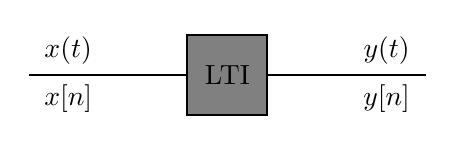
\begin{tikzpicture}
                \draw[thick] (0,0)  -- ++(2,0)node[near start, above] {$x(t)$} node[near start, below] {$x[n]$} node (s) [rectangle, draw=black, thick, fill=gray, minimum width=0.4in, minimum height = 0.4in,anchor=west] {LTI} (s.east) -- ++(2,0) node[near end, above] {$y(t)$} node[near end, below] {$y[n]$};
            \end{tikzpicture}
        \end{center}
        Decompose the input as
            \begin{equation*}
                x = a_1\phi_1 + a_2\phi_2 + \cdots \quad \text{linear combination of basic inputs}
            \end{equation*}
        Then
            \begin{equation*}
                y = a_1\psi_1 + a_2\psi_2 + \cdots \quad \text{linear combination of corresponding outputs}
            \end{equation*}

        Choose $\phi_k(t)$ or $\phi_k[n]$ such that
        \begin{itemize}
            \item Broad class of signals can be constructed, and
            \item Response to $\phi_k$s easy to compute.
        \end{itemize}
\end{frame}

\begin{frame}{Eigenfunction Property}
    \textbf{Continuous-Time}:\par
    $\phi_k(t) = e^{j\omega_k t}$:
    \begin{equation*}
        e^{j\omega_k t} \longrightarrow H(\omega_k) e^{j\omega_k t} \quad \text{(a scaled-version of the input)}
    \end{equation*}
    \textbf{``Discrete-Time'':}\pause
    \mode<beamer>
    {
        $\phi_k[n] = e^{j\omega_k n}$\par
        \begin{equation*}
            e^{j\omega_k n} \longrightarrow
            \underset{\mathclap{\tikz \node {$\uparrow$} node [below=3ex, text=red] {eigenfunction};}}{
            e^{j\omega_k n}
            }
            \underbrace{
            \sum_{r=-\infty}^{\infty} h[r]e^{-j\omega_k r}
            }_{\textcolor{red}{\text{eigenvalue}}}
        \end{equation*}
    }
\end{frame}


\begin{frame}{Discrete-Time Fourier Series}
    \mode<beamer>
    {
        \begin{columns}
            \column{0.48\textwidth}
                $x[n]$ periodic\par
                period $N$\par
                fundamental frequency $\omega_0 = \frac{2\pi}{N}$\par
                $e^{jk\omega_0 n} = e^{j(k+N)\omega_0 n}$\par
                \begin{equation*}
                    x[n] = \sum_k a_k e^{jk\omega_0 n}, \quad k = 0,1, 2, \dots, N-1.
                \end{equation*}
                \begin{equation*}
                    x[n] = \sum_{k=<N>} a_k e^{jk\omega_0 n}.
                \end{equation*}
                $N$ equations in $N$ unknowns.
                \begin{equation*}
                    a_k = \frac{1}{N}\sum_{<N>} x[n]e^{-jk\omega_0 n}.
                \end{equation*}
            \column{0.48\textwidth}
            \textbf{Continuous-Time}\par
            \begin{align*}
                x(t) &= \sum_{k=-\infty}^{\infty}a_k e^{jk\omega_0 t}\\
                a_k &= \frac{1}{T} \int_{T} x(t)e^{-jk\omega_0 t}dt
            \end{align*}
            \textbf{Discrete-Time Fourier Series}
            \mode<beamer>
            {

            \begin{align*}
                \text{Synthesis} &\\
                x[n] &= \sum_{k=<N>} a_k e^{jk\omega_0 n} = \sum_{k=<N>} a_k e^{jk(2\pi/N) n} .\\
                \text{Analysis} &\\
                a_k &= \frac{1}{N}\sum_{n=<N>} x[n]e^{-jk\omega_0 n}  = \frac{1}{N}\sum_{n=<N>} x[n]e^{-jk(2\pi/N) n}.
            \end{align*}
            }
        \end{columns}
    }
\end{frame}


\begin{frame}


    \mode<beamer>
    {
        \begin{columns}
            \column{0.48\textwidth}
            \textbf{Periodicity}
                \begin{equation*}
                    \begin{array}{lll}
                        x[n] & \text{periodic in } n & \text{true for CT}\\
                        e^{jk\omega_0 n} & \text{periodic in } n &\text{true for CT}\\
                        e^{jk\omega_0 n} & \text{periodic in } k &\text{not true for CT}\\
                        a_k &  \text{periodic in } k &\text{not true for CT}
                    \end{array}
                \end{equation*}
            \column{0.48\textwidth}
            \textbf{Convergence}\par
            Continuous-time:
            \begin{itemize}
                \item $x(t)$ square-integrable OR
                \item Dirichlet condition
            \end{itemize}
            Discrete-time
            \begin{equation*}
                x[n] = \sum_{k=<N>} a_k e^{jk\omega_0 n}.
            \end{equation*}
            \begin{equation*}
                \hat{x}[n] = \sum_{p \text{ terms}} a_k e^{jk\omega_0 n}.
            \end{equation*}
            $p = N$\par
            \begin{equation*}
                \hat{x}[n] \equiv x[n].
            \end{equation*}
            There is no issue of convergence in DT.
        \end{columns}
    }
\end{frame}

\begin{frame}{Example}
    Determine and sketch the DTFT of
    \begin{equation*}
        x[n] = 1 + \sin \omega_0 n + 3 \cos \omega_0 n + \cos\left(2\omega_0 n + \frac{\pi}{2}\right).
    \end{equation*}
    \pause
\end{frame}

\begin{frame}
    \begin{figure}
        \centering
        \begin{filecontents}{example52data.dat}
o reak akmag imak argak
-15 0 0 0 0
-14 0 0 0 0
-13 0 0 0 0
-12 0 0.5 -0.5 -1.57
-11 1.5 1.581 0.5 0.32
-10 1 1 0 0
-9 1.5 1.581 -0.5 -0.32
-8 0 0.5 0.5 1.57
-7 0 0 0 0
-6 0 0 0 0
-5 0 0 0 0
-4 0 0 0 0
-3 0 0 0 0
-2 0 0.5 -0.5 -1.57
-1 1.5 1.581 0.5 0.32
0  1 1 0 0
1 1.5 1.581 -0.5 -0.32
2 0 0.5 0.5 1.57
3 0 0 0 0
4 0 0 0 0
5 0 0 0 0
6 0 0 0 0
7 0 0 0 0
8 0 0.5 -0.5 -1.57
9 1.5 1.581 0.5 0.32
10  1 1 0 0
11 1.5 1.581 -0.5 -0.32
12 0 0.5 0.5 1.57
13 0 0 0 0
14 0 0 0 0
15 0 0 0 0
\end{filecontents}
\pgfplotstableread{example52data.dat}{\ninivina}

\begin{tikzpicture}[scale=0.6]	



    \begin{axis}[
    		name=axis1,
% 		y=1cm,
% 		x=1cm,
		 clip=false,
		 xmin=-12,xmax=12,
		 xlabel= $k$,
		 ylabel={$\mathfrak{Re}\{a_k\}$},
		 ymin=-1.5,ymax=2,
		axis lines=middle,
         	xtick={-10, 0, 10},
         	xticklabels={$-N$, $0$, $N$},
		 ytick={-1, 1},
		 yticklabels=\empty,
		 every axis x label/.style={at={(ticklabel* cs:1.05)}, anchor=west,},
		every axis y label/.style={at={(ticklabel* cs:1.05)}, anchor=south,},
     ]
	\addplot [red,very thick, ycomb] table [x={o}, y={reak}] {\ninivina};
	\node at (axis cs:0,1) [anchor= west] {\small $1$};
	\node at (axis cs:1,1.5) [anchor= west] {\small $\dfrac{3}{2}$};	
	\end{axis}
	
    \begin{axis}[
    		name=axis2,
    		at={($(axis1.east)+(10cm,0)$)},anchor= east,
% 		y=1cm,
% 		x=1cm,
		 clip=false,
		 xmin=-12,xmax=12,
		 xlabel= $k$,
		 ylabel={$|a_k|$},
		 ymin=-1.5,ymax=2,
		axis lines=middle,
         	xtick={-10, 0, 10},
         	xticklabels={$-N$, $0$, $N$},
		 ytick={-1, 1},
		 yticklabels=\empty,
		 every axis x label/.style={at={(ticklabel* cs:1.05)}, anchor=west,},
		every axis y label/.style={at={(ticklabel* cs:1.05)}, anchor=south,},
     ]
	\addplot [red,very thick, ycomb] table [x={o}, y={akmag}] {\ninivina};
	\node at (axis cs:0,1) [anchor= west] {\small $1$};
	\node at (axis cs:1,1.5) [anchor= west] {\small $\dfrac{\sqrt{10}}{2}$};		
	\node at (axis cs:2,.5) [anchor= west] {\small $\dfrac{1}{2}$};			
	\end{axis}	
	
    \begin{axis}[
    		name=axis3,
    		at={($(axis1.south east)+(0,-1.1cm)$)},anchor=north east,
% 		y=1cm,
% 		x=1cm,
		 clip=false,
		 xmin=-12,xmax=12,
		 xlabel= $k$,
		 ylabel={$\mathfrak{Im}\{a_k\}$},
		 ymin=-1.5,ymax=2,
		axis lines=middle,
         	xtick={-10, 0, 10},
         	xticklabels={$-N$, $0$, $N$},
		 ytick={-1, 1},
		 yticklabels=\empty,
		 every axis x label/.style={at={(ticklabel* cs:1.05)}, anchor=west,},
		every axis y label/.style={at={(ticklabel* cs:1.05)}, anchor=south,},
     ]
	\addplot [red,very thick, ycomb] table [x={o}, y={imak}] {\ninivina};
	\node at (axis cs:-1,.5) [anchor= east] {\small $\dfrac{1}{2}$};
	\node at (axis cs:1,-.5) [anchor= west] {\small $-\dfrac{1}{2}$};
	\end{axis}	
	
    \begin{axis}[
    		name=axis4,
    		at={($(axis2.south east)+(0,-1.1cm)$)},anchor=north east,
% 		y=1cm,
% 		x=1cm,
		 clip=false,
		 xmin=-12,xmax=12,
		 xlabel= $k$,
		 ylabel={$\angle a_k$},
		 ymin=-1.5,ymax=2,
		axis lines=middle,
         	xtick={-10, 0, 10},
         	xticklabels={$-N$, $0$, $N$},
		 ytick={-1, 1},
		 yticklabels=\empty,
		 every axis x label/.style={at={(ticklabel* cs:1.05)}, anchor=west,},
		every axis y label/.style={at={(ticklabel* cs:1.05)}, anchor=south,},
     ]
	\addplot [red,very thick, ycomb] table [x={o}, y={argak}] {\ninivina};
	\node at (axis cs:2,1.5) [anchor= west] {\small $\dfrac{\pi}{2}$};
	\node at (axis cs:-2,-1.5) [anchor= east] {\small $-\dfrac{\pi}{2}$};	
	\end{axis}		
\end{tikzpicture} 
    \end{figure}
\end{frame}

\begin{frame}{Example}
    Determine and sketch the DTFT of $x[n]$ of which is shown in the figure.
    \begin{figure}
        \centering
        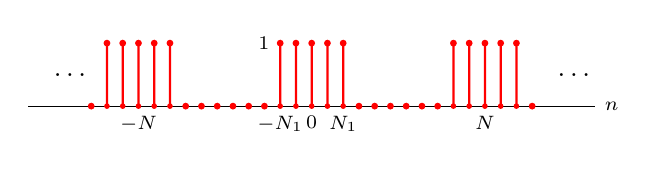
\begin{tikzpicture}[scale=0.8]

	\def\nmin{-13}
	\def\nmax{13}	
	
	\begin{scope}	
		\def\x{{0, 1, 1, 1, 1, 1, 0, 0, 0, 0, 0, 0, 1, 1, 1, 1, 1, 0, 0, 0, 0, 0, 0, 1, 1, 1, 1, 1, 0}}	

		\draw (-4.25, 0) -- (4.75, 0) node[anchor=west] {\scriptsize $n$};
		\foreach \n/\l in {-10/{-N}, -1/{-N_1}, 1/0, 3/{N_1}, 12/{N}}
		{
			\node at (\n/4, 0) [anchor=north] {\scriptsize $\l$};
		}
		\node at (-0.75,1) [anchor=west] {\scriptsize $1$};
		\node at (4,0.5) [anchor=west] {$\dots$};
		\node at (-4,0.5) [anchor=west] {$\dots$};
		
		\foreach \n in {0,1, ..., 28}
		{
			\pgfmathparse{\x[\n]}
			\edef\xn{\pgfmathresult}	
			\ifthenelse{\xn > 0}
			{
				\draw[red, thick, fill=red]  (\n/4 + \nmin/4, 0) -- ++(0, \xn) circle (1pt);% node[anchor=east] {\scriptsize $\xn$};
			}
			{
				\draw[red, fill=red] (\n/4+ \nmin/4,  0) circle (1pt);
			}
		}
	\end{scope}	
\end{tikzpicture}
    \end{figure}
    \pause
\end{frame}


\begin{frame}
    \begin{figure}
        \centering
        \begin{tikzpicture}[scale=0.3]	


    \begin{axis}[
    		name=axis1,
		y=1cm,
		x=1cm,
		 clip=false,
		 xmin=-3.5,xmax=10,
		 xlabel= $\omega$,
		 ylabel={$Na_k$},
		 ymin=-1.5,ymax=6,
		 axis lines=middle,
         	xtick={-3.1416, 3.1416, 6.2832},
         	xticklabels={$-\pi$, $\pi$, $2\pi$},
		 %ytick={-1, 1},
		 yticklabels=\empty,
		 every axis x label/.style={at={(ticklabel* cs:1.05)}, anchor=west,},
		every axis y label/.style={at={(ticklabel* cs:1.05)}, anchor=south,},
     ]
		\addplot [red, smooth, mark=none] table [x={o}, y={xo}] {g_dt_fs/figures/dtfs_square_N10.dat};
		\addplot [blue, ycomb, mark=*] table [x={o}, y={xo}] {g_dt_fs/figures/dtfs_square_stem_N10.dat};

		\node at (axis cs:10, 3) [anchor=east] { $N=10$ };
    \end{axis}


\pause
    \begin{axis}[
    	name=axis2,
    	at={($(axis1.south east)+(0,-1.1cm)$)},anchor=north east,
		y=1cm,
		x=1cm,
		 clip=false,
		 xmin=-3.5,xmax=10,
		 xlabel= $\omega$,
		 ylabel={$Na_k$},
		 ymin=-1.5,ymax=6,
		 axis lines=middle,
         	xtick={-3.1416, 3.1416, 6.2832},
         	xticklabels={$-\pi$, $\pi$, $2\pi$},
		 %ytick={-1, 1},
		 yticklabels=\empty,
		 every axis x label/.style={at={(ticklabel* cs:1.05)}, anchor=west,},
		every axis y label/.style={at={(ticklabel* cs:1.05)}, anchor=south,},
     ]
		\addplot [red, smooth, mark=none] table [x={o}, y={xo}] {g_dt_fs/figures/dtfs_square_N20.dat};%.
		\addplot [blue, ycomb, mark=*] table [x={o}, y={xo}] {g_dt_fs/figures/dtfs_square_stem_N20.dat};%.

		\node at (axis cs:10, 3) [anchor=east] { $N=20$ };
    \end{axis}

\pause
        \begin{axis}[
    	name=axis3,
    	at={($(axis2.south east)+(0,-1.1cm)$)},anchor=north east,
		y=1cm,
		x=1cm,
		 clip=false,
		 xmin=-3.5,xmax=10,
		 xlabel= $\omega$,
		 ylabel={$Na_k$},
		 ymin=-1.5,ymax=6,
		 axis lines=middle,
         	xtick={-3.1416, 3.1416, 6.2832},
         	xticklabels={$-\pi$, $\pi$, $2\pi$},
		 %ytick={-1, 1},
		 yticklabels=\empty,
		 every axis x label/.style={at={(ticklabel* cs:1.05)}, anchor=west,},
		every axis y label/.style={at={(ticklabel* cs:1.05)}, anchor=south,},
     ]
		\addplot [red, smooth, mark=none] table [x={o}, y={xo}] {g_dt_fs/figures/dtfs_square_N40.dat};
		\addplot [blue, ycomb, mark=*] table [x={o}, y={xo}] {g_dt_fs/figures/dtfs_square_stem_N40.dat};

		\node at (axis cs:10, 3) [anchor=east] { $N=40$ };
    \end{axis}

\end{tikzpicture} 
    \end{figure}   
\end{frame}

%\begin{frame}{}
%    \begin{enumerate}
%        \item
%    \end{enumerate}
%
%    \mode<beamer>
%    {
%        \begin{columns}
%            \column{0.48\textwidth}
%            \column{0.48\textwidth}
%        \end{columns}
%    }
%\end{frame} 